\section{PGG on Graphs}
\subsection{Proof of Concept: Replicator and Imitation Dynamics}

The paper chosen to replicate imitation and replicator dynamics was \cite{RN30}, which models a two-stage lottery game. Refer to \ref{Lottery} for a description of the game and the strategy space $C$. \\

The paper implemented agent--based replicator $(\alpha = 1)$ and imitation $(\alpha = 0)$ dynamics. After each round, every agent $i$ randomly chooses another agent $j$ from the population, and calculates $q_i$, \\

$$q_i = \Bigg[ \frac{|\pi_j - \pi_i|}{\Delta} \Bigg]^\alpha \mathbbm{1}_{\{\pi_j>\pi_i\}}, \quad  0 \leq \alpha \leq 1.$$

In the formulation, $\Delta$ scales the difference so that $0 \leq q_i \leq 1$, and $\Delta = 16$ in this two-stage lottery game. Each agent then changes from strategy $i$ to strategy $j$ if $q_i \geq r_i,$ $r_i \sim \mathsf{U}(0,1)$. \\

The simulated results were compared to the paper for $\alpha = 0, 1, 0.5$, and are shown below. \\

\FloatBarrier 
\begin{figure}[!h]
  \begin{subfigure}[b]{0.45\textwidth}
    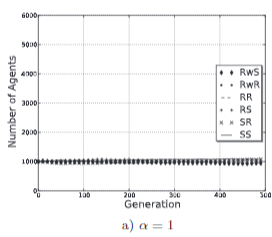
\includegraphics[width=\textwidth]{images/lottery1.png}
    \caption{Figure 5a from \cite{RN30}. The strategies SS, RR, SR, RS, R--WR, R--WS are represented by a solid line, crosses, plusses, dashes, dots and diamonds respectively. }
    \label{lottery1}
  \end{subfigure}
  \hfill
  \begin{subfigure}[b]{0.45\textwidth}
    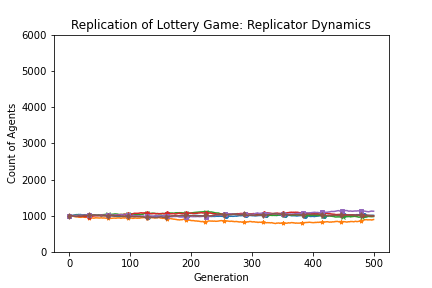
\includegraphics[width=1.25\textwidth]{images/lottery1_me.png}
    \caption{Replication of \ref{lottery1}. The strategies SS, RR, SR, RS, R--WR, R--WS are represented by blue circles, orange stars, green crosses, red pentagons, purple squares, and brown diamonds respectively.}
    \label{lottery1_me}
  \end{subfigure}
  \caption{Replication of Figure 5a from \cite{RN30}. The replication is successful, but these conditions do not provide anything interesting regarding replicator dynamics.} \label{lottery_comp0}
\end{figure} 
\FloatBarrier

\FloatBarrier 
\begin{figure}[!h]
  \begin{subfigure}[b]{0.45\textwidth}
    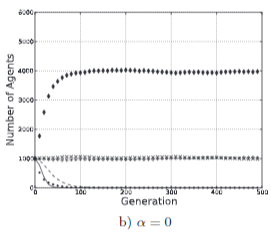
\includegraphics[width=\textwidth]{images/lottery2.png}
    \caption{Figure 5b from \cite{RN30}. The strategies SS, RR, SR, RS, R--WR, R--WS are represented by a solid line, crosses, plusses, dashes, dots and diamonds respectively. }
    \label{lottery2}
  \end{subfigure}
  \hfill
  \begin{subfigure}[b]{0.45\textwidth}
    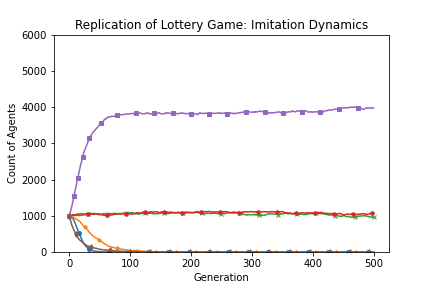
\includegraphics[width=1.25\textwidth]{images/lottery2_me.png}
    \caption{Replication of \ref{lottery2}. The strategies SS, RR, SR, RS, R--WR, R--WS are represented by blue circles, orange stars, green crosses, red pentagons, purple squares, and brown diamonds respectively. }
    \label{lottery2_me}
  \end{subfigure}
  \caption{Replication of Figure 5b from \cite{RN30}. The results are well replicated, and this model for imitation dynamics can be explored on other games.} \label{lottery_comp1}
\end{figure} 
\FloatBarrier



\FloatBarrier 
\begin{figure}[!h]
  \begin{subfigure}[b]{0.45\textwidth}
    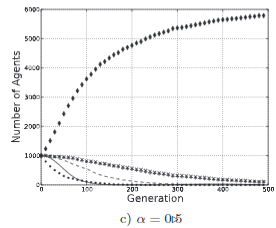
\includegraphics[width=\textwidth]{images/lottery3.png}
    \caption{Figure 5c from \cite{RN30}. The strategies SS, RR, SR, RS, R--WR, R--WS are represented by a solid line, crosses, plusses, dashes, dots and diamonds respectively. }
    \label{lottery3}
  \end{subfigure}
  \hfill
  \begin{subfigure}[b]{0.45\textwidth}
    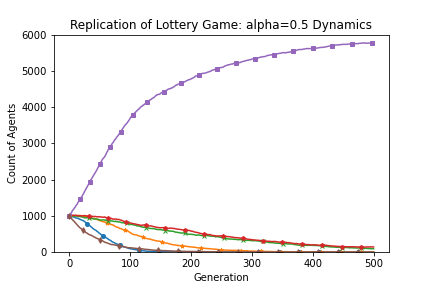
\includegraphics[width=1.25\textwidth]{images/lottery3_me.png}
    \caption{Replication of \ref{lottery3}. The strategies SS, RR, SR, RS, R--WR, R--WS are represented by blue circles, orange stars, green crosses, red pentagons, purple squares, and brown diamonds respectively. }
    \label{lottery3_me}
  \end{subfigure}
  \caption{Replication of Figure 5c from \cite{RN30}. This is neither true imitation or replicator dynamic, but provides an intermediary case.} \label{lottery_comp2}
\end{figure} 
\FloatBarrier

The replicator dynamics in Figure \ref{lottery_comp0} do not show any interesting trends, as each strategy has the same expected value, so $\mathbb E |\pi_i - \pi_j|^1 = 0$, for all $i,j \in C$. It is more interesting to examine the results when the lottery win probability $p$ is not 0.5. This was shown in Figure 6 from \cite{RN30}, and replicated below. For $p=0.4$, the expectation--maximising strategy is SS, but R--WS has an evolutionary advantage and takes over the population. This is supported by theoretical results in \cite{RN30}. Similarly, for $p=0.55$, the expectation--maximising strategy is RR, but R--WS also takes over the population.